% Politecnico di Milano (PoliMi) - School of Industrial and Information Engineering
%
% Last Revision: October 2021
%
% Copyright 2021 Politecnico di Milano, Italy. NC-BY

\documentclass{Configuration_Files/Template}

%------------------------------------------------------------------------------
%	REQUIRED PACKAGES AND  CONFIGURATIONS
%------------------------------------------------------------------------------

% CONFIGURATIONS
\usepackage{parskip} % For paragraph layout
\usepackage{setspace} % For using single or double spacing
\usepackage{emptypage} % To insert empty pages
\usepackage{multicol} % To write in multiple columns (executive summary)
\setlength\columnsep{15pt} % Column separation in executive summary
\setlength\parindent{0pt} % Indentation
\raggedbottom  

% PACKAGES FOR TITLES
\usepackage{titlesec}
% \titlespacing{\section}{left spacing}{before spacing}{after spacing}
\titlespacing{\section}{0pt}{3.3ex}{2ex}
\titlespacing{\subsection}{0pt}{3.3ex}{1.65ex}
\titlespacing{\subsubsection}{0pt}{3.3ex}{1ex}
\usepackage{color}

% PACKAGES FOR LANGUAGE AND FONT
\usepackage[english]{babel} % The document is in English  
\usepackage[utf8]{inputenc} % UTF8 encoding
\usepackage[T1]{fontenc} % Font encoding
\usepackage[11pt]{moresize} % Big fonts

% PACKAGES FOR IMAGES
\usepackage{graphicx}
\usepackage{transparent} % Enables transparent images
\usepackage{eso-pic} % For the background picture on the title page
\usepackage{subfig} % Numbered and caption subfigures using \subfloat.
\usepackage{tikz} % A package for high-quality hand-made figures.
\usetikzlibrary{}
\graphicspath{{./Images/}} % Directory of the images
\usepackage{caption} % Coloured captions
\usepackage{xcolor} % Coloured captions
\usepackage{amsthm,thmtools,xcolor} % Coloured "Theorem"
\usepackage{float}

% STANDARD MATH PACKAGES
\usepackage{amsmath}
\usepackage{amsthm}
\usepackage{amssymb}
\usepackage{amsfonts}
\usepackage{bm}
\usepackage[overload]{empheq} % For braced-style systems of equations.
\usepackage{fix-cm} % To override original LaTeX restrictions on sizes

% PACKAGES FOR TABLES
\usepackage{tabularx}
\usepackage{longtable} % Tables that can span several pages
\usepackage{colortbl}

% PACKAGES FOR ALGORITHMS (PSEUDO-CODE)
\usepackage{algorithm}
\usepackage{algorithmic}

% PACKAGES FOR REFERENCES & BIBLIOGRAPHY
\usepackage[colorlinks=true,linkcolor=black,anchorcolor=black,citecolor=black,filecolor=black,menucolor=black,runcolor=black,urlcolor=black]{hyperref} % Adds clickable links at references
\usepackage{cleveref}
\usepackage[square, numbers, sort&compress]{natbib} % Square brackets, citing references with numbers, citations sorted by appearance in the text and compressed
\bibliographystyle{abbrvnat} % You may use a different style adapted to your field

% OTHER PACKAGES
\usepackage{pdfpages} % To include a pdf file
\usepackage{afterpage}
\usepackage{lipsum} % DUMMY PACKAGE
\usepackage{fancyhdr} % For the headers
\fancyhf{}

% Input of configuration file. Do not change config.tex file unless you really know what you are doing. 
% Define blue color typical of polimi
\definecolor{bluepoli}{cmyk}{0.4,0.1,0,0.4}

% Custom theorem environments
\declaretheoremstyle[
  headfont=\color{bluepoli}\normalfont\bfseries,
  bodyfont=\color{black}\normalfont\itshape,
]{colored}

% Set-up caption colors
\captionsetup[figure]{labelfont={color=bluepoli}} % Set colour of the captions
\captionsetup[table]{labelfont={color=bluepoli}} % Set colour of the captions
\captionsetup[algorithm]{labelfont={color=bluepoli}} % Set colour of the captions

\theoremstyle{colored}
\newtheorem{theorem}{Theorem}[chapter]
\newtheorem{proposition}{Proposition}[chapter]

% Enhances the features of the standard "table" and "tabular" environments.
\newcommand\T{\rule{0pt}{2.6ex}}
\newcommand\B{\rule[-1.2ex]{0pt}{0pt}}

% Pseudo-code algorithm descriptions.
\newcounter{algsubstate}
\renewcommand{\thealgsubstate}{\alph{algsubstate}}
\newenvironment{algsubstates}
  {\setcounter{algsubstate}{0}%
   \renewcommand{\STATE}{%
     \stepcounter{algsubstate}%
     \Statex {\small\thealgsubstate:}\space}}
  {}

% New font size
\newcommand\numfontsize{\@setfontsize\Huge{200}{60}}

% Title format: chapter
\titleformat{\chapter}[hang]{
\fontsize{50}{20}\selectfont\bfseries\filright}{\textcolor{bluepoli} \thechapter\hsp\hspace{2mm}\textcolor{bluepoli}{|   }\hsp}{0pt}{\huge\bfseries \textcolor{bluepoli}
}

% Title format: section
\titleformat{\section}
{\color{bluepoli}\normalfont\Large\bfseries}
{\color{bluepoli}\thesection.}{1em}{}

% Title format: subsection
\titleformat{\subsection}
{\color{bluepoli}\normalfont\large\bfseries}
{\color{bluepoli}\thesubsection.}{1em}{}

% Title format: subsubsection
\titleformat{\subsubsection}
{\color{bluepoli}\normalfont\large\bfseries}
{\color{bluepoli}\thesubsubsection.}{1em}{}

% Shortening for setting no horizontal-spacing
\newcommand{\hsp}{\hspace{0pt}}

\makeatletter
% Renewcommand: cleardoublepage including the background pic
\renewcommand*\cleardoublepage{%
  \clearpage\if@twoside\ifodd\c@page\else
  \null
  \AddToShipoutPicture*{\BackgroundPic}
  \thispagestyle{empty}%
  \newpage
  \if@twocolumn\hbox{}\newpage\fi\fi\fi}
\makeatother

%For correctly numbering algorithms
\numberwithin{algorithm}{chapter}

%----------------------------------------------------------------------------
%	NEW COMMANDS DEFINED
%----------------------------------------------------------------------------

% EXAMPLES OF NEW COMMANDS
\newcommand{\bea}{\begin{eqnarray}} % Shortcut for equation arrays
\newcommand{\eea}{\end{eqnarray}}
\newcommand{\e}[1]{\times 10^{#1}}  % Powers of 10 notation

%----------------------------------------------------------------------------
%	ADD YOUR PACKAGES (be careful of package interaction)
%----------------------------------------------------------------------------

%----------------------------------------------------------------------------
%	ADD YOUR DEFINITIONS AND COMMANDS (be careful of existing commands)
%----------------------------------------------------------------------------

%----------------------------------------------------------------------------
%	BEGIN OF YOUR DOCUMENT
%----------------------------------------------------------------------------

\begin{document}

\fancypagestyle{plain}{%
\fancyhf{} % Clear all header and footer fields
\fancyhead[RO,RE]{\thepage} %RO=right odd, RE=right even
\renewcommand{\headrulewidth}{0pt}
\renewcommand{\footrulewidth}{0pt}}

%----------------------------------------------------------------------------
%	TITLE PAGE
%----------------------------------------------------------------------------

\pagestyle{empty} % No page numbers
\frontmatter % Use roman page numbering style (i, ii, iii, iv...) for the preamble pages

\puttitle{
	RASD document, % Title of the thesis
	name= Jacopo Piazzalunga, Mattia Piccinato, Gabriele Puglisi, % Author
	academicyear={2023-2024},  % Academic Year
} % These info will be put into your Title page 

%----------------------------------------------------------------------------
%	PREAMBLE PAGES: ABSTRACT (inglese e italiano), EXECUTIVE SUMMARY
%----------------------------------------------------------------------------
\startpreamble
\setcounter{page}{1} % Set page counter to 1

%----------------------------------------------------------------------------
%	LIST OF CONTENTS/FIGURES/TABLES/SYMBOLS
%----------------------------------------------------------------------------

% TABLE OF CONTENTS
\thispagestyle{empty}
\tableofcontents % Table of contents 
\thispagestyle{empty}
\cleardoublepage

%-------------------------------------------------------------------------
%	THESIS MAIN TEXT
%-------------------------------------------------------------------------
% In the main text of your thesis you can write the chapters in two different ways:
%
%(1) As presented in this template you can write:
%    \chapter{Title of the chapter}
%    *body of the chapter*
%
%(2) You can write your chapter in a separated .tex file and then include it in the main file with the following command:
%    \chapter{Title of the chapter}
%    \input{chapter_file.tex}
%
% Especially for long thesis, we recommend you the second option.

\addtocontents{toc}{\vspace{2em}} % Add a gap in the Contents, for aesthetics
\mainmatter % Begin numeric (1,2,3...) page numbering


% FIRST CHAPTER
% --------------------------------------------------------------------------
\chapter{Introduction}

\section{Purpose}

The purpose of the project CodeKataBattle (CKB) is to develop a platform where Students can practice coding together. Educators set up challenges (called Battles) within Tournaments, and Students work in teams to solve them. The platform checks their code automatically, giving scores based on how well it works, how quickly they finish, and how good their code quality is. Educators may optionally give extra scores by checking the work themselves, in a so-called Consolidation Stage which starts right after the end of every Battle. Students get ranked in Tournaments based on their scores obtained in teams, and can earn Badges for some achievements, in order to make learning programming more fun and competitive.

{\color{bluepoli}\rule{\linewidth}{0.1pt}}

\subsection{Goals}

{\color{bluepoli}\rule{\linewidth}{0.1pt}}

\begin{enumerate}
    \item[\textcolor{bluepoli}{G1}] Allows registered Students who enrolled according to the right modalities to participate in a Tournament of Battles and take part in its Battles.
    \item[\textcolor{bluepoli}{G2}] Allows registered Educators to manage Tournaments for which they have been granted permission.
    \item[\textcolor{bluepoli}{G3}] Allows registered Students who participate in a Tournament of Battles to be rewarded of different achievements.
    \item[\textcolor{bluepoli}{G4}] Allows registered Users to visualize information for which they have granted permission.
    \item[\textcolor{bluepoli}{G5}] Automates code evaluation process using GitHub Actions and some static analysis tools.
\end{enumerate}

{\color{bluepoli}\rule{\linewidth}{0.1pt}}

\section{Scope}

The main features which should be provided in order to achieve the aim of the project are:

\item \textcolor{bluepoli}{Creating Challenges:} Educators can make coding challenges (Battles) that Students can join, alone or in teams (groups), within the context of a Tournament.

\item \textcolor{bluepoli}{Using GitHub Actions for Code Submsissions:} Students are supposed to submit their code for a Battle in their GitHub repository, and the system must be informed of a new commit by a participating Student making use of GitHub Actions.

\item \textcolor{bluepoli}{Checking Code both Automatically and Manually:} The platform assigns a score to Students' code automatically, without the intervention of any Educator. Optionally, Educators may also decide to evaluate the code themselves.

\item \textcolor{bluepoli}{Rankings:} During each Battle, a live ranking of the involved teams is available, enabling participating Students to track their performance. Additionally, live Tournament rankings show how well each Student is performing in the Battles within a given Tournament.

\item \textcolor{bluepoli}{Badges for Achievements:} At the end of every Tournament, Students who achieved good results may be awarded with a special Badges, which are ruled by the Educator who created the Tournament.

The main goal is to help Students practice coding, giving them feedback and comparing their results to others.

\subsection{World phenomena}

{\color{bluepoli}\rule{\linewidth}{0.1pt}}

\begin{enumerate}
    \item[\textcolor{bluepoli}{WP1}] An Educator wants to create a Tournament competition.
    \item[\textcolor{bluepoli}{WP2}] A Student wants to participate in a Tournament competition.
    \item[\textcolor{bluepoli}{WP3}] A Student forks a Battle GitHub repo.
    \item[\textcolor{bluepoli}{WP4}] A Student sets up the update workflow using GitHub Actions.
    \item[\textcolor{bluepoli}{WP5}] An Educator wants to end a Tournament competition.
    \item[\textcolor{bluepoli}{WP6}] A User wants to visualize data about Tournaments, Battles, and Student profiles.
    \item[\textcolor{bluepoli}{WP7}] An Educator is given permission by another Educator to manage a Tournament.
\end{enumerate}

{\color{bluepoli}\rule{\linewidth}{0.1pt}}

\subsection{Shared phenomena}

{\color{bluepoli}\rule{\linewidth}{0.1pt}}

\subsubsection{Controlled by Machine}

\begin{enumerate}
    \item[\textcolor{bluepoli}{SP1}] The system notifies the Students about the creation of a Tournament.
    \item[\textcolor{bluepoli}{SP2}] The system notifies the groups about the creation of a Battle.
    \item[\textcolor{bluepoli}{SP3}] The system notifies the groups about the evaluation of a Battle.
    \item[\textcolor{bluepoli}{SP4}] The system notifies the Students about the end of a Tournament.s
    \item[\textcolor{bluepoli}{SP5}] The system shows some information about a Battle.
    \item[\textcolor{bluepoli}{SP6}] The system shows some information about a Tournament.
    \item[\textcolor{bluepoli}{SP7}] The system shows some information about a Student.
    \item[\textcolor{bluepoli}{SP8}] The system creates a GitHub repository containing the code Kata.
    \item[\textcolor{bluepoli}{SP9}] The system assigns the score to the code of a group.
    \item[\textcolor{bluepoli}{SP10}] The system assigns a Badge to a Student.
\end{enumerate}

\subsubsection{Controlled by World}

\begin{enumerate}
    \item[\textcolor{bluepoli}{SP11}] An Educator creates a Tournament of Battles.
    \item[\textcolor{bluepoli}{SP12}] An Educator defines Badges (see section 1.3) for the Tournament.
    \item[\textcolor{bluepoli}{SP13}] An Educator gives permission to another Educator to manage a Tournament.
    \item[\textcolor{bluepoli}{SP14}] An Educator creates a Battle.
    \item[\textcolor{bluepoli}{SP15}] A Student creates a group for a Battle.
    \item[\textcolor{bluepoli}{SP16}] A Student invites another Student to join the group they created.
    \item[\textcolor{bluepoli}{SP17}] A Student joins a group for a Battle.
    \item[\textcolor{bluepoli}{SP18}] An API call is received by the system when a commit is pushed.
    \item[\textcolor{bluepoli}{SP19}] An Educator closes a Battle.
    \item[\textcolor{bluepoli}{SP20}] An Educator closes a Tournament.
    \item[\textcolor{bluepoli}{SP21}] An Educator evaluates the code of a Student.
\end{enumerate}

{\color{bluepoli}\rule{\linewidth}{0.1pt}}

\section{Definitions, Acronyms, Abbreviations}

In this section some information about terminology is provided, in order to clarify terms, acronyms, and abbreviations used in the document, ensuring easy understanding and reference for readers.

{\color{bluepoli}\rule{\linewidth}{0.1pt}}

\subsection{Definitions}

{\color{bluepoli}\rule{\linewidth}{0.1pt}}

\item \textcolor{bluepoli}{Battle:} A Code Kata, that is, a challenge in which teams of players need to solve a problem in a specific coding language and submit their code to get a score according to the rules of the Battle.
\item \textcolor{bluepoli}{Tournament:} A competition composed of many Battles in which participants' overall score is the sum of all the scores obtained in every Battle they participated in, individually or in team with other players.
\item \textcolor{bluepoli}{Student:} The User which takes part into the Tournaments of Battles.
\item \textcolor{bluepoli}{Educator:} The User which organizes Tournaments of Battles to which the Students can participate and who manages every aspect about them.
\item \textcolor{bluepoli}{Consolidation stage:} The Consolidation Stage is the phase of a Battle which starts as soon as the submission deadline expires, during which the Educators who manage the Tournament can eventually assign an additional score to every team, which will be summed to the score previously assigned by the platform.
\item \textcolor{bluepoli}{Badge:} A Badge is an achievement marker related to a certain Tournament, obtained by Students if they satisfied the specific conditions defined by the Educator during the creation process of the Tournament.

{\color{bluepoli}\rule{\linewidth}{0.1pt}}

\subsection{Acronyms}

{\color{bluepoli}\rule{\linewidth}{0.1pt}}

\item \textcolor{bluepoli}{CK:} Code Kata, that is, a Battle.
\item \textcolor{bluepoli}{CKB:} Code Kata Battle, that is, the name of the platform.

{\color{bluepoli}\rule{\linewidth}{0.1pt}}

\subsection{Abbreviations}

{\color{bluepoli}\rule{\linewidth}{0.1pt}}

\item \textcolor{bluepoli}{WPn:} n-th World Phenomena
\item \textcolor{bluepoli}{SPn:} n-th Shared Phenomena
\item \textcolor{bluepoli}{Gn:} n-th Goal
\item \textcolor{bluepoli}{Dn:} n-th Domain Assumption
\item \textcolor{bluepoli}{Rn:} n-th Requirement

{\color{bluepoli}\rule{\linewidth}{0.1pt}}

\section{Revision history}

\section{Reference Documents}

\item \textcolor{bluepoli}{Assignment document A.Y. 2023/2024}\\
(”Requirement Engineering and Design Project: goal, schedule and rules”)
\item \textcolor{bluepoli}{Software Engineering 2 A.Y. 2023/2024 Slides}\\
(Lecture slides provided during the course)

{\color{bluepoli}\rule{\linewidth}{0.1pt}}

\section{Document Structure}

This document is composed of six sections:

\item \textcolor{bluepoli}{1st Chapter:} We begin by presenting the problem statement and outlining the system's objectives. In the scope subsection, we offer insights into the various real-world and shared phenomena that the system addresses. Finally, we provide essential resources for readers, including definitions and abbreviations, to facilitate a comprehensive understanding of this document.
\item \textcolor{bluepoli}{2nd Chapter:} We offer a comprehensive overview of the system, including insights into User profiles and their primary functions. Additionally, we present domain diagrams to illustrate system components and describe various scenarios. Finally, we establish the key domain assumptions underpinning the system's operation
\item \textcolor{bluepoli}{3rd Chapter:} We delineate the system's requirements, encompassing both functional and non-functional aspects. In addition, we present use case diagrams that illustrate system interactions, accompanied by detailed descriptions of each use case and related sequence diagrams. Lastly, we establish a clear mapping of these requirements to both system goals and use cases for comprehensive understanding.
\item \textcolor{bluepoli}{4th Chapter:} We provide a formal analysis of the system to be with Alloy.
\item \textcolor{bluepoli}{5th Chapter:} We provide an estimate of the effort spent by each group member.
\item \textcolor{bluepoli}{6th Chapter:} We provide a list of the references used in this document.

{\color{bluepoli}\rule{\linewidth}{0.1pt}}


% SECOND CHAPTER
% --------------------------------------------------------------------------
\chapter{Overall Description}

\section{Product perspective}

CKB is a platform meant to help Students practice coding through CKs. Educators set up these Battles for teams of Students to compete in coding exercises using different programming languages like Java or Python. Each CK has a description and tasks to complete, but Students must write the actual code themselves and make sure it passes certain tests before a deadline.

Educators decide the Battle rules, like team sizes and deadlines. Once the Battles are set, Students form teams and get their own GitHub pages. They need to use GitHub Actions to automate checking their code, which the CKB evaluates.

Scores are given automatically based on how well the code works, how quickly it's finished after signing up, and its quality. Educators might also add scores based on other things. CKB updates the team standings as the Battle goes on and gives final scores when it's done.

Students' scores from different Battles add up to give a total for the whole Tournament. Also, the platform gives out Badges for achievements and participation that everyone can see on a Student's profile.

{\color{bluepoli}\rule{\linewidth}{0.1pt}}

\subsection{Scenarios}

{\color{bluepoli}\rule{\linewidth}{0.1pt}}

\item \textcolor{bluepoli}{1st Scenario: Signing up and logging in} User signs up, logs out and signs in: The User Mark opens the platform and starts the signing up procedure, fills the required data and completes the signign up procedure. Then he logs out to be sure that everything went fine, and a few seconds later he logs in again.
\item \textcolor{bluepoli}{2nd Scenario: Creating a Tournament} Kevin the Educator creates a Tournament and sets the subscription deadline. He creates the Badges for the Tournament, specifying their title and rules by using the specific language, referring to existing variables in the system.
\item \textcolor{bluepoli}{3rd Scenario: Giving permission to manage a Tournament} Kevin the Educator gives the permission to his colleague Lara to create further Battles within the context of the Tournament.
\item \textcolor{bluepoli}{4th Scenario: Creating a Battle in a Tournament} Kevin the Educator creates a first Battle for the Tournament and sets registration and submission deadlines, providing a brief textual description, the software project and the set of test cases; then, he sets minimum and maximum number of members per group and specifies the additional mandatory configurations for scoring and whether the manual evaluation is needed. All the Students in the platform are notified. 
\item \textcolor{bluepoli}{5th Scenario: Joining a Tournament} Jim the Student subscribes to a certain Tournament Battle, forming a new group for an existing Battle. Right after, Jim invites Kyle, another Student, which accepts Jim’s invite to join his existing group.
\item \textcolor{bluepoli}{6th Scenario: Starting Battle} The registration deadline of a Battle expires, then the system creates a GitHub repository and sends the link to all the registered Students.
\item \textcolor{bluepoli}{7th Scenario: Forking the Battle repository}: Jim the Student forks the repository related to the Battle. He then sets up the automated workflow.
\item \textcolor{bluepoli}{8th Scenario: Pushing a commit for a Battle} Jim the Student pushes a commit (before the expiration of the submission deadline). The system pulls the commit, executes the runnable to test the outcome, computes the mandatory aspects’ (functional aspects, timeliness and sources quality) score between 0 and 100 and updates both the Battle score of the group and the Battle ranking if the new commit score is better than the previous best one for the group.
\item \textcolor{bluepoli}{9th Scenario: Ending Battle} The submission deadline of a Battle expires. The Battle enters the Consolidation Stage. Kevin the Educator assigns the personal optional scores. Then the system assigns the score for every group in the Battle ranking, and the personal score for every Student. The system notifies all the participating Students as soon as the Battle ranking has been updated. The system updates the Tournament ranking adding the single Battle score, for each Student.
\item \textcolor{bluepoli}{10th Scenario: Ending Tournament} Kevin the Educator ends a Tournament. Any running Battle is stopped. The system computes the scores for the last commits which were pushed and waiting to be computed and notifies all the Students. The personal scores are updated by the system. Badges are assigned to the Students by the system.
\item \textcolor{bluepoli}{11th Scenario: Visualizing content} The User Michael visualizes the current Battle ranking before the submission deadline expires. He also visualizes the current list of Tournaments, picks one of them and visualizes its ranking. Finally, he picks the first Student in the Tournament ranking and visualizes their profile, in order to see their Badges.

{\color{bluepoli}\rule{\linewidth}{0.1pt}}

\subsection{Class Diagram}

{\color{bluepoli}\rule{\linewidth}{0.1pt}}
Qui\\
{\color{bluepoli}\rule{\linewidth}{0.1pt}}

\subsection{State Charts}

{\color{bluepoli}\rule{\linewidth}{0.1pt}}
Qui\\
{\color{bluepoli}\rule{\linewidth}{0.1pt}}

\section{Product functions}

The platform CKB offers several key functions:

\item \textcolor{bluepoli}{Battles and Tournaments Creation} Educators can create coding challenges (Battles) within Tournaments, specifying details like descriptions, team sizes, deadlines, scoring configurations and, eventually, Badges.
\item \textcolor{bluepoli}{Student Participation} On the other hand, Students can join such Tournaments and take part in Battles, individually or in teams. 
\item \textcolor{bluepoli}{GitHub Integration} The system allows the Students to perform code submissions just by pushing their code on GitHub, thanks to automated workflows triggered by GitHub Actions service.
\item \textcolor{bluepoli}{Automated Evaluation} The platform automatically evaluates Student code based on test cases, timeliness, and code quality using external static analysis tools.
\item \textcolor{bluepoli}{Scoring and Ranking} It continuously updates team rankings during Battles and provides overall Tournament rankings at the end of each Battle.
\item \textcolor{bluepoli}{Badges and Recognition} Educators define Badges which can be obtained by Students, serving as recognition for accomplishments and participation to a certain Tournament.
\item \textcolor{bluepoli}{Manual Optional Evaluation} Educators can manually evaluate Students' work and assign additional scores at the end of every Battle.

{\color{bluepoli}\rule{\linewidth}{0.1pt}}

\subsection{Requirements}

{\color{bluepoli}\rule{\linewidth}{0.1pt}}

\begin{enumerate}
    \item[\textcolor{bluepoli}{R1}] The system must allow an unregistered Educator to sign up.
    \item[\textcolor{bluepoli}{R2}] The system must allow an unregistered Student to sign up.
    \item[\textcolor{bluepoli}{R3}] The system must allow a registered User to log in.
    \item[\textcolor{bluepoli}{R4}] The system must allow registered Educators to start the creation process of a Tournament of Battles.
    \item[\textcolor{bluepoli}{R5}] The system must provide registered Educators of a list of Tournament-related statistics for the Badges definition, during the Tournament creation process.
    \item[\textcolor{bluepoli}{R6}] The system must provide registered Educators of a specific language which lets them define the Badges, during the Tournament creation process.
    \item[\textcolor{bluepoli}{R7}] The system must allow registered Educators to grant other registered Educators the permission to manage the Tournament, during the Tournament creation process.
    \item[\textcolor{bluepoli}{R8}] The system must allow registered Educators to end the creation process of a Tournament that they started themselves.
    \item[\textcolor{bluepoli}{R9}] The system must be able to send notifications to every registered User.
    \item[\textcolor{bluepoli}{R10}] The system must allow a registered Educator to create a Battle in a Tournament if and only if he is the creator of the Tournament or if he was granted the permission to by the latter.
    \item[\textcolor{bluepoli}{R11}] The system must allow a registered Student to create a group for a Battle in a Tournament.
    \item[\textcolor{bluepoli}{R12}] The system must allow a registered Student to accept an invitation to a group for a Battle in a Tournament.
    \item[\textcolor{bluepoli}{R13}] The system must allow registered Students to see the list of ongoing Tournaments and join any of those if its subscription deadline is not expired yet.
    \item[\textcolor{bluepoli}{R14}] The system must allow registered Students who are enrolled in a Battle to perform code submissions.
    \item[\textcolor{bluepoli}{R15}] The system must be provided of proper APIs to let registered Students perform code submissions through GitHub Actions.
    \item[\textcolor{bluepoli}{R16}] The system must update the Battle ranking when a valid code submission is performed.
    \item[\textcolor{bluepoli}{R17}] The system must set the Consolidaton Stage of a Battle when its submission deadline expires.
    \item[\textcolor{bluepoli}{R18}] The system must let Educators to end the Consolidaton Stage of a Battle if and only if he is the creator of the Tournament or if he was granted the permission to by the latter.
    \item[\textcolor{bluepoli}{R19}] The system must update Tournament ranking when a Battle exits the Consolidaton Stage.
    \item[\textcolor{bluepoli}{R20}] The system must let Educators who are either the creator of the Tournament or who have been granted the permission to by the latter to close a Tournament if and only if there is no Battle such that either their subscription or submission deadline is not expired yet or such that they are still in the Consolidaton Stage.
    \item[\textcolor{bluepoli}{R21}] The system must assign an achievements’ Badge for a given Tournament to any Student who satisfied the conditions defined by the creator of the Tournament.
    \item[\textcolor{bluepoli}{R22}] The system must allow every User to see the Badges which were ever obtained by a given Student.
    \item[\textcolor{bluepoli}{R23}] The system must notify every registered Student about the creation of a new Tournament.
    \item[\textcolor{bluepoli}{R24}] The system must notify every registered Student about the creation of a new Battle within a Tournament they are enrolled in.
    \item[\textcolor{bluepoli}{R25}] The system must notify every registered Student about the end of a Battle they are participating in.
    \item[\textcolor{bluepoli}{R26}] The system must notify every registered Student about the end of a Tournament they are enrolled in.
\end{enumerate}

{\color{bluepoli}\rule{\linewidth}{0.1pt}}

\section{User characteristics}

In the CKB platform, a User can be either a Student or an Educator, each with distinct roles and motivations.

\item \textcolor{bluepoli}{Students} They join Battles to practice coding in a collaborative environment, aiming to enhance their programming skills through practical challenges, seeking to measure their performance against peers and track their progress. Students can achieve recognition by obtaining Badges within the context of a Tournament. Students are often notified about new activities that they may want to join, such as a new Tournament, or a new Battle within the context of a Tournament that they are enrolled in.
\item \textcolor{bluepoli}{Educators} They set up and manage the coding challenges, individually or cooperating with other Educators. They act as facilitators, creating Battles within Tournaments to engage Students in practical exercises. Educators may want to personally evaluate Students' code submissions, in order to reward particularly brilliant solutions or to penalize major mistakes. Additionally, they are responsible for defining Badge criteria, which act as a motivating factor.

{\color{bluepoli}\rule{\linewidth}{0.1pt}}

\section{Assumptions, dependencies and constraints}

This section serves as a comprehensive overview of critical factors which must be considered during the implementation of the platform. It consolidates the foundational assumptions made during project planning and highlights eventual dependencies.

{\color{bluepoli}\rule{\linewidth}{0.1pt}}

\subsection{Domain Assumptions}

{\color{bluepoli}\rule{\linewidth}{0.1pt}}t

\begin{enumerate}
    \item[\textcolor{bluepoli}{D1}] The User must have a working Internet connection.
    \item[\textcolor{bluepoli}{D2}] The Students who participate to a Battle properly set up the GitHub Action for code submissions.
    \item[\textcolor{bluepoli}{D3}] The Users always receive every notification which is sent by the system.
    \item[\textcolor{bluepoli}{D4}] The availability of the static analysis tools utilized for the code evaluation process is consistent.
    \item[\textcolor{bluepoli}{D5}] The availability of GitHub Actions service is consistent.
\end{enumerate}

{\color{bluepoli}\rule{\linewidth}{0.1pt}}

\subsection{Dependencies}

{\color{bluepoli}\rule{\linewidth}{0.1pt}}

The static analysis tools which provide a score based on the quality level of each code submission can either be implemented or integrated in the system. Similarly, the notification provider can either be implemented or integrated in the system. For the registration process, a verification email must be sent by the system to let Users successfully sign up, thus requiring the integration of an e-mail service.

{\color{bluepoli}\rule{\linewidth}{0.1pt}}


% THIRD CHAPTER
% --------------------------------------------------------------------------
\chapter{Specific requirements}

\section{External Interface Requirements}
Qui\\
{\color{bluepoli}\rule{\linewidth}{0.1pt}}

\subsection{User Interfaces}
{\color{bluepoli}\rule{\linewidth}{0.1pt}}
Qui\\
{\color{bluepoli}\rule{\linewidth}{0.1pt}}

\subsection{Hardware Interfaces}
{\color{bluepoli}\rule{\linewidth}{0.1pt}}
Qui\\
{\color{bluepoli}\rule{\linewidth}{0.1pt}}

\subsection{Software Interfaces}
{\color{bluepoli}\rule{\linewidth}{0.1pt}}
Qui\\
{\color{bluepoli}\rule{\linewidth}{0.1pt}}

\subsection{Communication Interfaces}
{\color{bluepoli}\rule{\linewidth}{0.1pt}}
Qui\\
{\color{bluepoli}\rule{\linewidth}{0.1pt}}

\section{Design Constraints}
Qui\\
{\color{bluepoli}\rule{\linewidth}{0.1pt}}

\section{Software System Attributes}
Qui\\
{\color{bluepoli}\rule{\linewidth}{0.1pt}}

\subsection{Reliability}
{\color{bluepoli}\rule{\linewidth}{0.1pt}}
Qui\\
{\color{bluepoli}\rule{\linewidth}{0.1pt}}

\subsection{Availability}
{\color{bluepoli}\rule{\linewidth}{0.1pt}}
Qui\\
{\color{bluepoli}\rule{\linewidth}{0.1pt}}

\subsection{Security}
{\color{bluepoli}\rule{\linewidth}{0.1pt}}
Qui\\
{\color{bluepoli}\rule{\linewidth}{0.1pt}}

\subsection{Maintainability}
{\color{bluepoli}\rule{\linewidth}{0.1pt}}
Qui\\
{\color{bluepoli}\rule{\linewidth}{0.1pt}}

\subsection{Portability}
{\color{bluepoli}\rule{\linewidth}{0.1pt}}
Qui\\
{\color{bluepoli}\rule{\linewidth}{0.1pt}}

% FOURTH CHAPTER
% --------------------------------------------------------------------------
\chapter{Formal analysis using alloy}

\section{Objectives of the analysis}

\item In this section, a presentation of the formal modelling activity that has been done using the Alloy formal notation. The main goal of this activity is to formally describe the domain and properties of the system to be.
\item In particular, the main objective of this activity is to model and formally represent Educators, Students, Tournaments, Battles and Badges, as well as the main constraints which regard such entities.
\item In order to ensure straightforward comprehension of the following, each constraint and entity will be annotated in natural language, along with any predicates and assertions which have been verified.

{\color{bluepoli}\rule{\linewidth}{0.1pt}}

\section{Alloy Code}

\item // -------------- Definition of auxiliar entities -------------- //
\\
\item // Defined in order to model the deadlines
\item sig Time \{\\
timestamp: Int\\
\}\{\\
timestamp >= 0\\
\}
\\
\item // Defined in order to model any flag, such as whether a Battle is in the Consolidation Stage
\item abstract sig Boolean \{\}
\item one sig True extends Boolean \{\}
\item one sig False extends Boolean \{\}
\\
\item // -------------- Definition of game components -------------- //
\\
\item // Defined in order to model the score of a team in a Battle and the score of a Student in a Tournament
\item sig Score \{\\
value: Int\\
\}\{\\
value >= 0\\
\}
\\
\item // Defined in order to model the rank of a team in a Battle and the rank of a Student in a Tournament
\item sig Rank \{\\
value: Int\\
\}\{\\
value >= 1\\
\}
\\
\item // Defined in order to model the Tournament
\item sig Tournament \{\\
managers: some Educator,\\
subscription\_deadline: one Time,\\
battles: set Battle,\\
scores: Student -> one Score,\\
ranks: Student -> one Rank,
badges: set Badge,\\
achievements: Student -> set BadgeRule\\
\}
\\
\item // Defined in order to model the Battle (unnecessary to model the programming language)
\item sig Battle \{\\
tournament: one Tournament,\\
teams: Student -> some Student,\\
scores: Student -> one Score,\\
ranks: Student -> one Rank,\\
subscription\_deadline: one Time,\\
submission\_deadline: one Time,\\
consolidation\_stage: one Boolean\\
\}
\\
\item // Defined in order to model the Badge (unnecessary to model the title)
\item sig BadgeRule \{\\
\}
\item sig Badge \{\\
rule: one BadgeRule\\
\}
\\
\item // -------------- Definition of actors -------------- //
\\
\item // Defined in order to model the nature of Student and Educator as Users
\item abstract sig User \{\}
\\
\item // Defined in order to model the Student
\item sig Student extends User \{\\
badges: set Badge\\
\}
\\
\item // Defined in order to model the Educator
\item sig Educator extends User\{\\
\}
\\
\item //  -------------- Facts -------------- //
\\
\item // Tournaments: A student must both have a score and a rank, if a student has higher score than another student than it has a lower rank (e.g. 1st is lower than 2nd), only achievements of Badges which relate to existing Badges for the Tournament are stored, a Student has one only score, a Student has one only rank
\item fact TournamentFact \{\\
    all t1: Tournament | all s: Student | some sc: Score | some r: Rank | ( sc in s.(t1.scores) ) => ( r in s.(t1.ranks) ) and ( r in s.(t1.ranks) => sc in s.(t1.scores) )\\
    all t2: Tournament | all s1, s2: Student | ( ( s1.(t2.ranks).value < s2.(t2.ranks).value ) <=> ( s1.(t2.scores).value > s2.(t2.scores).value ) )\\
    all t3: Tournament | all s3: Student | all b: Badge | ( b.rule in s3.(t3.achievements) ) => ( b in t3.badges )\\
    all t4: Tournament | all disj sc1, sc2: Score | some s: Student | ( sc1 in s.(t4.scores) ) => not ( sc2 in s.(t4.scores) )\\
    all t5: Tournament | all disj r1, r2: Rank | some s: Student | ( r1 in s.(t5.ranks) ) => not ( r2 in s.(t5.ranks) )\\
\}
\\
\item // Battles: The subscription deadline must expire before the submission deadline, teams relationships are symmetrical, teams relationships are reflexive, if a Student s1 is in team with a Student s2 and not with a Student s3 then s2 is not in team with s3, Students in the same team have same score and rank, a Student has one only score, a Student has one only rank
\item fact BattleFact \{\\
    all b: Battle | b.subscription\_deadline.timestamp < b.submission\_deadline.timestamp\\
    all b1: Battle | all s1, s2: Student | s2 in s1.(b1.teams) <=> s1 in s2.(b1.teams)\\
    all b2: Battle | all s: Student | s in s.(b2.teams)\\
    all b3: Battle | all s3, s4, s5: Student | ( ( s4 in s3.(b3.teams) )  and ( not ( s5 in s3.(b3.teams) ) ) ) => ( not (s4 in s5.(b3.teams) ) )\\
    all b4: Battle | all s6, s7: Student | s7 in s6.(b4.teams) => ( ( s6.(b4.scores).value = s7.(b4.scores).value ) and ( s6.(b4.ranks).value = s7.(b4.scores).value ) )\\
    all b5: Battle | all disj sc1, sc2: Score | some s8: Student | ( sc1 in s8.(b5.scores) ) => ( not ( sc2 in s8.(b5.scores) ) )\\
    all b6: Battle | all disj r1, r2: Rank | some s9: Student | ( r1 in s9.(b6.ranks) ) => ( not ( r2 in s9.(b6.ranks) ) )\\
\}
\\
\item // A student must have obtained the Badges in some Tournament
\item fact studentObtainedBadges \{\\
one t: Tournament | all s: Student, b: Badge | b in s.badges => b.rule in s.(t.achievements)\\
\}
\\
\item // -------------- Predicates and assertions -------------- //
\\
\item //  1. A basic example
\item pred show \{\\
some b: Battle | some t: Tournament | b in t.battles\\
\}
\item run show
\begin{figure}[H]
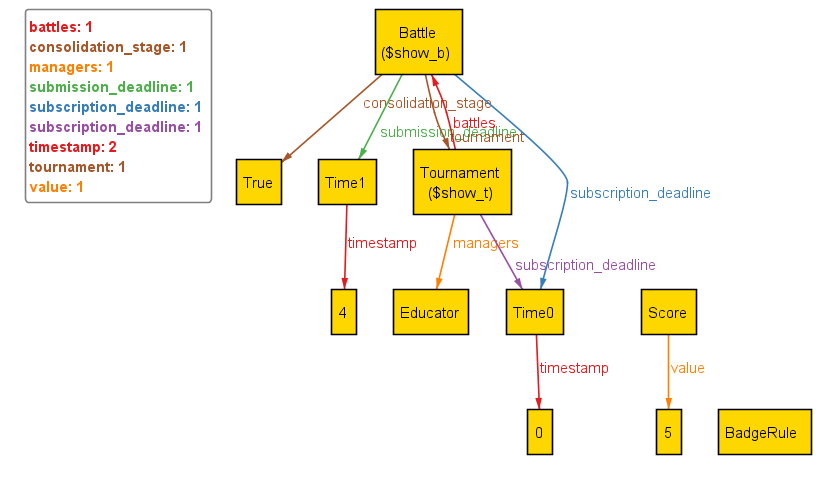
\includegraphics[scale = 0.7]{RASD_latex/Images/Alloy/1Model.png}\\
\centering
\end{figure}
\begin{figure}[H]
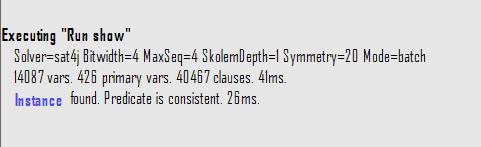
\includegraphics[scale = 0.7]{RASD_latex/Images/Alloy/1Outcome.png}
\centering
\end{figure}
\\
\\
\\
\item //  2. An example to show that a higher position in the ranking corresponds to a lower score
\item pred RankingExample \{\\
    some disj b1, b2: Battle | some t: Tournament | b1 in t.battles and b2 in t.battles\\
    some disj s3, s4: Student | some b3: Battle | ( not ( s3 in s4.(b3.teams) ) ) and ( s3.(b3.ranks).value != s4.(b3.ranks).value )\\
    some r1, r2: Rank | r1.value = 1 and r2.value = 2\\
    some sc1, sc2: Score | ( sc1. value = 5 ) and ( sc2.value = 6 )\\
\}
\item run RankingExample
\begin{figure}[H]
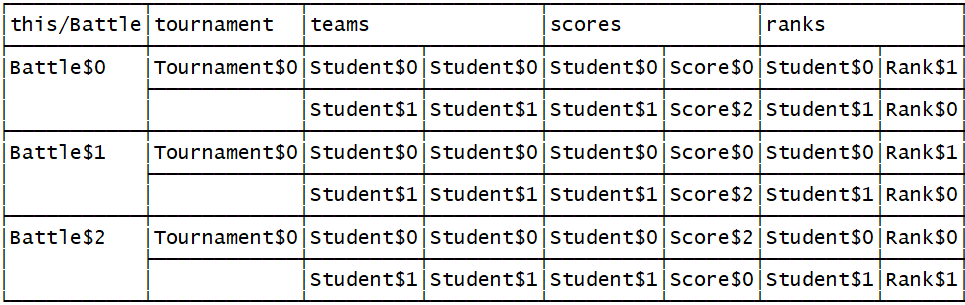
\includegraphics[scale = 0.7]{RASD_latex/Images/Alloy/2Table1.png}\\
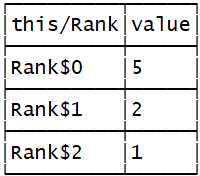
\includegraphics[scale = 0.7]{RASD_latex/Images/Alloy/2Table2.png}\\
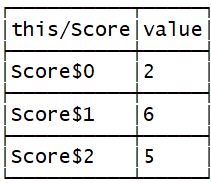
\includegraphics[scale = 0.7]{RASD_latex/Images/Alloy/2Table3.png}\\
\centering
\end{figure}
\begin{figure}[H]
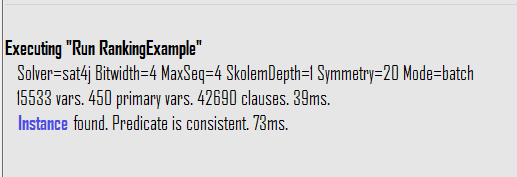
\includegraphics[scale = 0.7]{RASD_latex/Images/Alloy/2Outcome.png}\\
\centering
\end{figure}
\\
\\
\\
\item //  3. Ensuring that Badges obtained by students must be existed in some Tournaments (in this model, Tournament can both represent both a running one or a finished one)
\item assert ExistingBadges \{
    all b: Badge | all s: Student | some t: Tournament | ( b in s.badges ) => ( b in t.badges)\\
\}
\item check ExistingBadges
\begin{figure}[H]
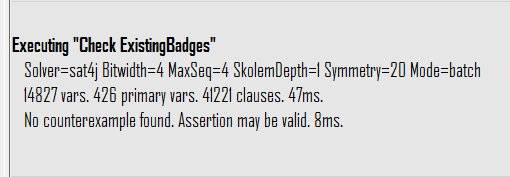
\includegraphics[scale = 0.7]{RASD_latex/Images/Alloy/3Outcome.png}\\
\centering
\end{figure}
\\
\\
\\
{\color{bluepoli}\rule{\linewidth}{0.1pt}}

% FIFTH CHAPTER
% --------------------------------------------------------------------------
\chapter{Effort spent}

% SIXTH CHAPTER
% --------------------------------------------------------------------------
\chapter{References}


\end{document}
